\chapter{Cinemática del punto}\label{ch:b1:point-kinematics}

El vagón de una montaña rusa entra en el rizo a \qty{90}{km/h}, frena
mientras sube, queda suspendido un instante arriba y sale rugiendo; sus
pasajeros se sienten aplastados contra el asiento abajo y casi ingrávidos
arriba. Describir ese trayecto --- dónde está el vagón, con qué rapidez se
mueve, cómo gira y cambia su \omterm{def:b1:point-kinematics:velocity}{velocidad} --- es cinemática, y hace falta
algo más que las $x$, $y$, $z$ de una carretera recta: \omterm{def:b1:point-kinematics:cylindrical}{coordenadas polares}
para todo lo que gira y un sistema que viaje con el propio vagón. Este
capítulo monta esas herramientas, demuestra las fórmulas de la \omterm{def:b1:point-kinematics:velocity}{velocidad} y
la \omterm{def:b1:point-kinematics:velocity}{aceleración} en cada una de ellas y las aplica a los movimientos que
invocará cualquier capítulo posterior: circular, helicoidal, armónico y el
movimiento a lo largo de una curva cualquiera.

\section{Posición, velocidad, aceleración}

\begin{definition}[Sistema de referencia; posición; trayectoria]\label{def:b1:point-kinematics:frame}
\index{sistema de referencia}\index{vector de posición}\index{trayectoria}\index{punto material}
Un \emph{sistema de referencia} es un sólido tomado como fijo (el
laboratorio, la Tierra, un tren) junto con un reloj. Un \emph{punto
material} $M$ --- un cuerpo cuyo tamaño es irrelevante para el movimiento
estudiado --- queda situado en cada instante por su \emph{vector de
posición} $\vect{OM}(t)$ desde un origen $O$ ligado al sistema; la curva
que describe $M$ es su \emph{trayectoria}. El movimiento es siempre
movimiento \emph{respecto de un sistema}: un mismo pasajero está en reposo
en el tren y en movimiento en la estación.
\end{definition}

\begin{definition}[Velocidad y aceleración]\label{def:b1:point-kinematics:velocity}
\index{velocidad}\index{aceleración}
La \emph{velocidad} y la \emph{aceleración} de $M$ en el sistema son
\[
\vect v = \frac{\dd\vect{OM}}{\dd t}, \qquad
\vect a = \frac{\dd\vect v}{\dd t} = \frac{\dd^2\vect{OM}}{\dd t^2},
\]
derivadas de funciones vectoriales: la derivada de un vector se obtiene
derivando sus componentes en una base \emph{fija en el sistema}. La
velocidad es tangente a la \omterm{def:b1:point-kinematics:frame}{trayectoria} y apunta en el sentido del
movimiento; su norma $v$ es la \emph{rapidez}. Unidades:
\unit{m/s}, \unit{m/s^2}.
\end{definition}

\begin{proposition}[Coordenadas cartesianas]\label{prop:b1:point-kinematics:cartesian}
\index{coordenadas cartesianas}
Con una base ortonormal fija $(\vect e_x, \vect e_y, \vect e_z)$ y
$\vect{OM} = x\,\vect e_x + y\,\vect e_y + z\,\vect e_z$,
\[
\vect v = \dot x\,\vect e_x + \dot y\,\vect e_y + \dot z\,\vect e_z, \qquad
\vect a = \ddot x\,\vect e_x + \ddot y\,\vect e_y + \ddot z\,\vect e_z,
\]
donde el punto denota $\dd/\dd t$.
\end{proposition}

\begin{proof}
Los vectores de la base son constantes; solo varían las componentes.
\end{proof}

\begin{example}[Proyectil]\label{ex:b1:point-kinematics:projectile}
Lanzada desde $O$ con rapidez $v_0$ y un ángulo $\alpha$ sobre la
horizontal, las coordenadas de una pelota (dinámica, capítulo siguiente)
son $x = v_0\cos\alpha\,t$, $z = v_0\sin\alpha\,t - \tfrac12 gt^2$.
Entonces $\vect v = v_0\cos\alpha\,\vect e_x + (v_0\sin\alpha - gt)\vect e_z$
y $\vect a = -g\vect e_z$: la \omterm{def:b1:point-kinematics:velocity}{aceleración} es constante mientras la
\omterm{def:b1:point-kinematics:velocity}{velocidad} gira; en el vértice ($\dot z = 0$, $t = v_0\sin\alpha/g$) la
\omterm{def:b1:point-kinematics:velocity}{velocidad} es horizontal y la \omterm{def:b1:point-kinematics:velocity}{aceleración} perpendicular a ella. Eliminando
$t$: $z = x\tan\alpha - gx^2/(2v_0^2\cos^2\alpha)$, una parábola.
\end{example}

\begin{omfigure}
\begin{tikzpicture}[font=\small, x=1cm, y=1cm]
  \draw[-Stealth] (0,0) -- (6.8,0) node[right] {$x$};
  \draw[-Stealth] (0,0) -- (0,3.6) node[above] {$z$};
  \node[below left] at (0,0) {$O$};
  \draw[omDef, thick, domain=0:6, samples=80] plot (\x, {2.2*\x - 0.3667*\x*\x});
  % point at x=1.5: z=2.2*1.5-0.3667*2.25=3.3-0.825=2.475 ; slope = 2.2 - 0.7333*1.5 = 1.1
  \fill[omThm] (1.5,2.475) circle (1.6pt); \node[above left] at (1.5,2.475) {$M$};
  \draw[-Stealth, omThm, thick] (1.5,2.475) -- ++(1.0,1.1) node[above right] {$\vect v$};
  \draw[-Stealth, omProp, thick] (1.5,2.475) -- ++(0,-1.2) node[right] {$\vect a = \vect g$};
  \draw[-Stealth, omExo] (0,0) -- (1.5,2.475); \node[omExo, left] at (0.72,1.45) {$\vect{OM}$};
  % apex at x=3: z=6.6-3.3=3.3
  \fill[omThm] (3,3.3) circle (1.6pt);
  \draw[-Stealth, omThm, thick] (3,3.3) -- ++(1.2,0);
  \draw[-Stealth, omProp, thick] (3,3.3) -- ++(0,-1.2);
\end{tikzpicture}

{\small La parábola de un proyectil: la \omterm{def:b1:point-kinematics:velocity}{velocidad} es tangente a la
\omterm{def:b1:point-kinematics:frame}{trayectoria} y gira, y la \omterm{def:b1:point-kinematics:velocity}{aceleración} $\vect g$ es constante. En el vértice
la \omterm{def:b1:point-kinematics:velocity}{velocidad} y la \omterm{def:b1:point-kinematics:velocity}{aceleración} son perpendiculares: la rapidez es
momentáneamente estacionaria mientras la dirección sigue cambiando.}
\end{omfigure}

\section{Coordenadas cilíndricas}

\begin{definition}[Coordenadas cilíndricas y base local]\label{def:b1:point-kinematics:cylindrical}
\index{coordenadas cilíndricas}\index{coordenadas polares}\index{base local}
El punto $M$ queda situado por $r \geq 0$ (distancia al eje $z$), el
ángulo $\theta$ que forma su proyección sobre el plano $xy$ con
$\vect e_x$, y $z$: $\vect{OM} = r\,\vect e_r + z\,\vect e_z$, donde
\[
\vect e_r = \cos\theta\,\vect e_x + \sin\theta\,\vect e_y, \qquad
\vect e_\theta = -\sin\theta\,\vect e_x + \cos\theta\,\vect e_y,
\]
y $\vect e_z$ forman la \emph{base local} $(\vect e_r, \vect e_\theta,
\vect e_z)$, ortonormal y directa, que \emph{se mueve con $M$}. En el
plano ($z$ fijo) son las \emph{coordenadas polares} $(r, \theta)$.
\end{definition}

\begin{lemma}[Derivadas de la base local]\label{lem:b1:point-kinematics:basisderiv}
\[
\frac{\dd\vect e_r}{\dd t} = \dot\theta\,\vect e_\theta, \qquad
\frac{\dd\vect e_\theta}{\dd t} = -\dot\theta\,\vect e_r, \qquad
\frac{\dd\vect e_z}{\dd t} = \vect 0 .
\]
\end{lemma}

\begin{proof}
Derívense las componentes: $\dd\vect e_r/\dd t = \dot\theta(-\sin\theta\,
\vect e_x + \cos\theta\,\vect e_y) = \dot\theta\vect e_\theta$, y de forma
análoga para $\vect e_\theta$. La derivada de un vector unitario que gira
es perpendicular a él y de norma igual a la \omterm{cor:b1:point-kinematics:circular}{velocidad angular}.
\end{proof}

\begin{theorem}[Velocidad y aceleración en coordenadas cilíndricas]\label{thm:b1:point-kinematics:cylindrical}
\[
\vect v = \dot r\,\vect e_r + r\dot\theta\,\vect e_\theta + \dot z\,\vect e_z,
\qquad
\vect a = \big(\ddot r - r\dot\theta^2\big)\vect e_r
+ \big(r\ddot\theta + 2\dot r\dot\theta\big)\vect e_\theta + \ddot z\,\vect e_z .
\]
\end{theorem}

\begin{proof}
Derívese $\vect{OM} = r\vect e_r + z\vect e_z$ con el lema:
$\vect v = \dot r\vect e_r + r\dot\theta\vect e_\theta + \dot z\vect e_z$.
Derívese otra vez: $\ddot r\vect e_r + \dot r\dot\theta\vect e_\theta +
\dot r\dot\theta\vect e_\theta + r\ddot\theta\vect e_\theta - r\dot\theta^2
\vect e_r + \ddot z\vect e_z$; agrúpese.
\end{proof}

\begin{omfigure}
\begin{tikzpicture}[font=\small, x=1cm, y=1cm]
  \draw[-Stealth] (0,0) -- (5.2,0) node[right] {$x$};
  \draw[-Stealth] (0,0) -- (0,3.6) node[above] {$y$};
  \node[below left] at (0,0) {$O$};
  \coordinate (M) at (35:3.4);
  \draw[omExo] (0,0) -- (M); \fill[omThm] (M) circle (1.6pt); \node[below right, xshift=2pt] at (M) {$M$};
  \node[omExo] at (20:1.9) {$r$};
  \draw (0.9,0) arc (0:35:0.9); \node at (17:1.15) {$\theta$};
  \draw[-Stealth, omDef, very thick] (M) -- ++(35:1.1) node[right] {$\vect e_r$};
  \draw[-Stealth, omDef, very thick] (M) -- ++(125:1.0) node[left] {$\vect e_\theta$};
  % trajectory sketch: spiral
  \draw[omThm, thick, domain=5:75, samples=50, variable=\t] plot ({(2.2+0.0343*\t)*cos(\t)},{(2.2+0.0343*\t)*sin(\t)});
  \draw[-Stealth, omThm, thick] (M) -- ++(100:1.6) node[above right] {$\vect v$};
\end{tikzpicture}

{\small \omterm{def:b1:point-kinematics:cylindrical}{Coordenadas polares}: la \omterm{def:b1:point-kinematics:cylindrical}{base local} $(\vect e_r, \vect e_\theta)$
gira con $M$; la \omterm{def:b1:point-kinematics:velocity}{velocidad} tiene una parte radial $\dot r$ y una parte
ortorradial $r\dot\theta$. Aquí la \omterm{def:b1:point-kinematics:frame}{trayectoria} (roja) se enrolla hacia
fuera, de modo que $\dot r > 0$ y $\vect v$ se inclina hacia fuera
respecto de la tangente a la circunferencia.}
\end{omfigure}

\begin{corollary}[Movimiento circular]\label{cor:b1:point-kinematics:circular}
\index{movimiento circular}\index{aceleración centrípeta}\index{velocidad angular}
Sobre una circunferencia de radio $R$ ($r = R$, $z = 0$), con
\emph{\omterm{cor:b1:point-kinematics:circular}{velocidad angular}} $\omega = \dot\theta$:
\[
\vect v = R\omega\,\vect e_\theta, \qquad
\vect a = -R\omega^2\,\vect e_r + R\dot\omega\,\vect e_\theta
= -\frac{v^2}{R}\,\vect e_r + \frac{\dd v}{\dd t}\,\vect e_\theta .
\]
Para el \omterm{cor:b1:point-kinematics:circular}{movimiento circular} \emph{uniforme} ($\omega$ constante), la
\omterm{def:b1:point-kinematics:velocity}{aceleración} es puramente \emph{centrípeta}, de norma $v^2/R = R\omega^2$,
aunque la rapidez sea constante.
\end{corollary}

\begin{proof}
Hágase $\dot r = \ddot r = 0$ en el teorema; $v = R\omega$.
\end{proof}

\begin{example}[Dos circunferencias]\label{ex:b1:point-kinematics:circles}
Un coche recorre una rotonda de radio \qty{20}{m} a \qty{36}{km/h}
(\qty{10}{m/s}): $a = v^2/R = \qty{5.0}{m/s^2}$, medio $g$, dirigida hacia
el centro --- lo que han de aportar los neumáticos. La Luna
($R = \qty{3.84e8}{m}$, $T = \qty{27.3}{d}$): $\omega = 2\pi/T =
\qty{2.66e-6}{rad/s}$, $a = R\omega^2 = \qty{2.7e-3}{m/s^2}$, la
$3600$\textsuperscript{a} parte de $g$ en la superficie terrestre, a
sesenta radios terrestres --- la comparación que hizo Newton (\cref{ch:b1:central-forces}).
\end{example}

\section{Coordenadas esféricas}

\begin{definition}[Coordenadas esféricas]\label{def:b1:point-kinematics:spherical}
\index{coordenadas esféricas}
El punto $M$ queda situado por su distancia $r = OM$, la \emph{colatitud}
$\theta \in [0, \pi]$ entre $\vect{OM}$ y $\vect e_z$, y el \emph{azimut}
$\varphi$ de su proyección sobre el plano $xy$:
$\vect{OM} = r\,\vect e_r$ con
\[
\vect e_r = \sin\theta\cos\varphi\,\vect e_x + \sin\theta\sin\varphi\,\vect e_y + \cos\theta\,\vect e_z ;
\]
$\vect e_\theta$ (tangente al meridiano, hacia los $\theta$ crecientes) y
$\vect e_\varphi$ (tangente al paralelo) completan la \omterm{def:b1:point-kinematics:cylindrical}{base local}
ortonormal. Sobre la Tierra, $\theta$ es $90^\circ$ menos la latitud y
$\varphi$ es la longitud.
\end{definition}

\begin{proposition}[Velocidad en coordenadas esféricas]\label{prop:b1:point-kinematics:sphericalv}
\[
\vect v = \dot r\,\vect e_r + r\dot\theta\,\vect e_\theta + r\sin\theta\,\dot\varphi\,\vect e_\varphi .
\]
\end{proposition}

\begin{proof}
$\dd\vect e_r/\dd t = \dot\theta\,\vect e_\theta + \sin\theta\,\dot\varphi\,
\vect e_\varphi$: el primer término es la rotación en el plano meridiano
(como en el caso polar) y el segundo la rotación alrededor de $\vect e_z$
a razón de $\dot\varphi$ de un vector cuya distancia al eje vale
$\sin\theta$. Después $\vect v = \dd(r\vect e_r)/\dd t$. Este año no se
necesita la \omterm{def:b1:point-kinematics:velocity}{aceleración}.
\end{proof}

\begin{omfigure}
\begin{tikzpicture}[font=\small, x=1cm, y=1cm, scale=0.95]
  \draw[-Stealth] (0,0) -- (-2.4,-0.96) node[below left] {$x$};
  \draw[-Stealth] (0,0) -- (4.2,0) node[right] {$y$};
  \draw[-Stealth] (0,0) -- (0,3.6) node[above] {$z$};
  \node[below right] at (0,0) {$O$};
  \coordinate (M) at (1.4,2.4);
  \coordinate (P) at (1.4,-0.3);
  \draw[omExo] (0,0) -- (M); \fill[omThm] (M) circle (1.6pt); \node[above left] at (M) {$M$};
  \draw[dashed] (M) -- (P); \draw[dashed] (0,0) -- (P);
  \node[omExo] at (0.45,1.45) {$r$};
  \draw (0,1.0) arc (90:60:1.0); \node at (0.3,1.25) {$\theta$};
  \draw (-0.74,-0.3) arc (202:348:0.8); \node at (0.15,-1.05) {$\varphi$};
  \draw[-Stealth, omDef, very thick] (M) -- ++(0.45,0.77) node[above] {$\vect e_r$};
  \draw[-Stealth, omDef, very thick] (M) -- ++(0.77,-0.45) node[right] {$\vect e_\theta$};
  \draw[-Stealth, omDef, very thick] (M) -- ++(0.84,0.33) node[right] {$\vect e_\varphi$};
\end{tikzpicture}

{\small \omterm{def:b1:point-kinematics:spherical}{Coordenadas esféricas} $(r, \theta, \varphi)$ y su \omterm{def:b1:point-kinematics:cylindrical}{base local}:
$\vect e_r$ radial, $\vect e_\theta$ a lo largo del meridiano (hacia el
sur en un globo terráqueo) y $\vect e_\varphi$ a lo largo del paralelo
(hacia el este).}
\end{omfigure}

\section{La base de Frenet}

\begin{definition}[Abscisa curvilínea; base de Frenet]\label{def:b1:point-kinematics:frenet}
\index{abscisa curvilínea}\index{base de Frenet}\index{radio de curvatura}
A lo largo de una \omterm{def:b1:point-kinematics:frame}{trayectoria}, la \emph{abscisa curvilínea} $s(t)$ es la
longitud de arco desde un punto de referencia, contada algebraicamente;
$v = \dot s$. En $M$, la tangente unitaria $\vect T = \dd\vect{OM}/\dd s$
apunta hacia los $s$ crecientes; el \emph{radio de curvatura} $\rho > 0$ y
la normal unitaria $\vect N$, dirigida hacia el lado cóncavo (el centro de
curvatura), quedan definidos por
\[
\frac{\dd\vect T}{\dd s} = \frac{1}{\rho}\,\vect N .
\]
$(\vect T, \vect N)$ es la \emph{base de Frenet}; $\rho = \infty$ en una
recta y $\rho = R$ en una circunferencia de radio $R$.
\end{definition}

\begin{theorem}[Aceleración en la base de Frenet]\label{thm:b1:point-kinematics:frenet}
\index{aceleración tangencial}\index{aceleración normal}
\[
\vect v = v\,\vect T, \qquad
\vect a = \frac{\dd v}{\dd t}\,\vect T + \frac{v^2}{\rho}\,\vect N .
\]
La componente \emph{tangencial} $\dd v/\dd t$ mide con qué rapidez cambia
la rapidez; la componente \emph{normal} $v^2/\rho$, siempre hacia el
centro de curvatura, con qué rapidez gira la dirección. El movimiento es
uniforme si y solo si $\vect a \perp \vect v$; es rectilíneo si y solo si
$\vect a \parallel \vect v$.
\end{theorem}

\begin{proof}
$\vect v = (\dd\vect{OM}/\dd s)(\dd s/\dd t) = v\vect T$. Entonces $\vect a =
\dot v\vect T + v\,\dd\vect T/\dd t = \dot v\vect T + v(\dd\vect T/\dd s)\dot s
= \dot v\vect T + (v^2/\rho)\vect N$. Que $\dd\vect T/\dd s \perp \vect T$
se sigue de derivar $\vect T\cdot\vect T = 1$.
\end{proof}

\begin{omfigure}
\begin{tikzpicture}[font=\small, x=1cm, y=1cm]
  \draw[omDef, thick, domain=-2.6:3.2, samples=80] plot (\x, {0.22*\x*\x - 0.05*\x*\x*\x});
  % point at x=1: y=0.17 ; slope = 0.44-0.15=0.29 -> T direction angle 16.2 deg
  \coordinate (M) at (1,0.17);
  \fill[omThm] (M) circle (1.6pt); \node[below right] at (M) {$M$};
  \draw[-Stealth, omThm, very thick] (M) -- ++(16.2:1.2) node[right] {$\vect T$};
  \draw[-Stealth, omThm, very thick] (M) -- ++(106.2:1.2) node[above] {$\vect N$};
  % center of curvature: curvature kappa = y''/(1+y'^2)^{3/2}: y''=0.44-0.3=0.14 ; (1+0.0841)^1.5=1.129 -> kappa=0.124 -> rho=8.06 (too big) ; draw just arrow to C off-figure shortened
  \draw[dashed, omExo] (M) -- ++(106.2:3.0) node[above] {hacia $C$, a distancia $\rho$};
  \draw[-Stealth, omProp, thick] (M) -- ++(16.2:0.8) ++(0,0) -- ++(106.2:1.0);
  \draw[-Stealth, omProp, very thick] (M) -- ($(M)+(16.2:0.8)+(106.2:1.0)$) node[above right] {$\vect a$};
  \node[omProp, font=\footnotesize] at ($(M)+(16.2:0.95)+(0,-0.25)$) {$\dot v$};
  \node[omProp, font=\footnotesize] at ($(M)+(16.2:0.8)+(106.2:0.5)+(0.25,0)$) {$v^2/\rho$};
\end{tikzpicture}

{\small La \omterm{def:b1:point-kinematics:frenet}{base de Frenet} en un punto de una curva: $\vect T$ a lo largo
del movimiento y $\vect N$ hacia el centro de curvatura $C$. La
\omterm{def:b1:point-kinematics:velocity}{aceleración} se descompone en una parte tangencial $\dot v\vect T$
(acelerar o frenar) y una parte normal $(v^2/\rho)\vect N$ (girar).}
\end{omfigure}

\begin{example}[Frenar en una curva]\label{ex:b1:point-kinematics:bend}
Un coche a \qty{90}{km/h} (\qty{25}{m/s}) en una curva de radio
\qty{100}{m} frena a \qty{2.0}{m/s^2}: $a_T = \qty{-2.0}{m/s^2}$, $a_N = 625/100 =
\qty{6.25}{m/s^2}$, $a = \sqrt{4 + 39} = \qty{6.6}{m/s^2}$. Domina la
parte normal: una curva es ante todo un giro, y la adherencia de los
neumáticos (capítulo siguiente) limita $\sqrt{a_T^2 + a_N^2}$, razón por
la cual se frena \emph{antes} de la curva.
\end{example}

\section{Movimientos habituales}

\begin{proposition}[Movimiento rectilíneo uniformemente acelerado]\label{prop:b1:point-kinematics:uarm}
\index{movimiento uniformemente acelerado}
Sobre un eje, con $\ddot x = a$ constante, a partir de $x_0$ y $v_0$:
$v = v_0 + at$, $x = x_0 + v_0t + \tfrac12 at^2$, y
$v^2 - v_0^2 = 2a(x - x_0)$.
\end{proposition}

\begin{proof}
Intégrese dos veces; elimínese $t$ entre las dos primeras relaciones.
\end{proof}

\begin{proposition}[Movimiento helicoidal]\label{prop:b1:point-kinematics:helix}
\index{movimiento helicoidal}
$r = R$, $\theta = \omega t$, $z = v_zt$ (con $R$, $\omega$, $v_z$
constantes): la rapidez $v = \sqrt{R^2\omega^2 + v_z^2}$ es constante, la
\omterm{def:b1:point-kinematics:velocity}{aceleración} $\vect a = -R\omega^2\vect e_r$ es centrípeta y de norma
constante, y el \omterm{def:b1:point-kinematics:frenet}{radio de curvatura} vale $\rho = v^2/a = R(1 + v_z^2/R^2\omega^2) > R$.
\end{proposition}

\begin{proof}
\cref{thm:b1:point-kinematics:cylindrical} con $\dot r = 0$,
$\ddot\theta = 0$, $\ddot z = 0$; movimiento uniforme, luego $\vect a$ es
puramente normal y $v^2/\rho = R\omega^2$.
\end{proof}

\begin{proposition}[Movimiento armónico]\label{prop:b1:point-kinematics:harmonic}
\index{movimiento armónico}
$x = A\cos(\omega t + \varphi)$: $\dot x = -A\omega\sin(\omega t + \varphi)$,
$\ddot x = -\omega^2 x$. La \omterm{def:b1:point-kinematics:velocity}{velocidad} se adelanta a la posición en un
cuarto de periodo y la \omterm{def:b1:point-kinematics:velocity}{aceleración} es opuesta a la posición; $v_{\max} =
A\omega$, $a_{\max} = A\omega^2$. Es la proyección sobre un diámetro de un
\omterm{cor:b1:point-kinematics:circular}{movimiento circular} uniforme de radio $A$ y \omterm{cor:b1:point-kinematics:circular}{velocidad angular} $\omega$.
\end{proposition}

\begin{proof}
Derívese; para la proyección, tómese $x = A\cos\theta$ con $\theta =
\omega t + \varphi$.
\end{proof}

\begin{method}[Elegir las coordenadas]\label{met:b1:point-kinematics:choose}
\begin{itemize}
  \item Movimiento rectilíneo o parabólico, con \omterm{def:b1:point-kinematics:velocity}{aceleración} constante:
        cartesianas.
  \item Movimiento en torno a un eje o a un punto (circunferencias,
        espirales, órbitas, plataformas giratorias): cilíndricas o
        polares; la base se mueve, así que úsese
        \cref{thm:b1:point-kinematics:cylindrical} y nunca una derivación
        ingenua de las componentes.
  \item Una curva dada (una vía, una curva, un rizo) cuando se conoce la
        ley de rapidez: Frenet, que separa el ``cuán deprisa'' del ``hacia dónde''.
\end{itemize}
Sea cual sea la elección, $\vect v$ y $\vect a$ son vectores que dependen
del sistema, y un resultado solo está completo si se nombra el sistema.
\end{method}

\section{Ejercicios}

\begin{exercise}[$\star$]\label{exo:b1:point-kinematics:1}
Un coche arranca del reposo con $x(t) = 2.0\,t^2$ (unidades SI). \omterm{def:b1:point-kinematics:velocity}{Velocidad}
y \omterm{def:b1:point-kinematics:velocity}{aceleración} en $t = \qty{3.0}{s}$; distancia recorrida en los primeros
\qty{5}{s}; tiempo hasta alcanzar \qty{100}{km/h}.
\end{exercise}

\begin{exercise}[$\star$]\label{exo:b1:point-kinematics:2}
Un punto se mueve en un plano con $r = \qty{2.0}{m}$ y $\theta = 3.0\,t$
(rad, SI). Dense $\vect v$ y $\vect a$ en la base polar, sus normas y la
naturaleza del movimiento.
\end{exercise}

\begin{exercise}[$\star$]\label{exo:b1:point-kinematics:3}
Un punto del ecuador ($R = \qty{6.37e6}{m}$, día sidéreo \qty{86164}{s}):
rapidez y \omterm{def:b1:point-kinematics:velocity}{aceleración} en el sistema geocéntrico. Compárese la \omterm{def:b1:point-kinematics:velocity}{aceleración}
con $g$.
\end{exercise}

\begin{exercise}[$\star$]\label{exo:b1:point-kinematics:4}
Se lanza una pelota con $v_0 = \qty{12}{m/s}$ y $\alpha = 40^\circ$; sus
coordenadas son las de \cref{ex:b1:point-kinematics:projectile}. Hállense
el tiempo hasta el vértice, la altura máxima, el alcance y la \omterm{def:b1:point-kinematics:velocity}{velocidad} al
llegar al suelo.
\end{exercise}

\begin{exercise}[$\star\star$]\label{exo:b1:point-kinematics:5}
Un ciclista a \qty{10}{m/s} entra en una curva de radio \qty{25}{m} y
acelera a \qty{1.0}{m/s^2}. Dense $\vect a$ en la \omterm{def:b1:point-kinematics:frenet}{base de Frenet} y su
norma; ¿y al cabo de \qty{5}{s} con la misma \omterm{def:b1:point-kinematics:velocity}{aceleración} en la misma curva?
\end{exercise}

\begin{exercise}[$\star\star$]\label{exo:b1:point-kinematics:6}
Un punto sigue la espiral $r = b\theta$, $\theta = \omega t$ (con $b$ y
$\omega$ constantes). Calcúlense $\vect v$, la rapidez y $\vect a$ en la
base polar. ¿De dónde procede el término $2\dot r\dot\theta$?
\end{exercise}

\begin{exercise}[$\star\star$]\label{exo:b1:point-kinematics:7}
Hélice: $R = \qty{2.0}{m}$, $\omega = \qty{1.0}{rad/s}$, $v_z = \qty{0.50}{m/s}$.
Rapidez, \omterm{def:b1:point-kinematics:velocity}{aceleración}, paso de la hélice y \omterm{def:b1:point-kinematics:frenet}{radio de curvatura}.
\end{exercise}

\begin{exercise}[$\star\star$]\label{exo:b1:point-kinematics:8}
Un pistón se mueve como $x = 0.10\cos(10t)$ (SI). Dense $v_{\max}$,
$a_{\max}$, las relaciones de fase entre $x$, $v$ y $a$, y las posiciones
en las que $\abs v$ y $\abs a$ son máximos.
\end{exercise}

\begin{exercise}[$\star\star$]\label{exo:b1:point-kinematics:9}
A partir de $\vect e_r = \cos\theta\,\vect e_x + \sin\theta\,\vect e_y$,
dedúzcanse $\dd\vect e_r/\dd t$ y $\dd\vect e_\theta/\dd t$ y, después, la
\omterm{def:b1:point-kinematics:velocity}{velocidad} y la \omterm{def:b1:point-kinematics:velocity}{aceleración} polares de \cref{thm:b1:point-kinematics:cylindrical}.
\end{exercise}

\begin{exercise}[$\star\star\star$]\label{exo:b1:point-kinematics:10}
Para el proyectil de \cref{ex:b1:point-kinematics:projectile}, hállese el
\omterm{def:b1:point-kinematics:frenet}{radio de curvatura} de la \omterm{def:b1:point-kinematics:frame}{trayectoria} en el vértice y en el punto de
lanzamiento (úsese la componente normal de $\vect g$). ¿Cuál es menor, y
por qué?
\end{exercise}

\begin{exercise}[$\star\star\star$]\label{exo:b1:point-kinematics:11}
Una rueda de radio $R$ rueda sin deslizar con rapidez $v$; un punto de su
borde tiene coordenadas $x = vt - R\sin(vt/R)$, $y = R - R\cos(vt/R)$ (una
cicloide). Calcúlense su \omterm{def:b1:point-kinematics:velocity}{velocidad} y su \omterm{def:b1:point-kinematics:velocity}{aceleración}; muéstrese que al
tocar el suelo su \omterm{def:b1:point-kinematics:velocity}{velocidad} se anula y su \omterm{def:b1:point-kinematics:velocity}{aceleración} vale $v^2/R$ hacia
arriba; hállese su rapidez en lo alto.
\end{exercise}

\begin{exercise}[$\star\star\star$]\label{exo:b1:point-kinematics:12}
Una persona camina hacia fuera a lo largo de un radio de una plataforma
que gira con $\omega$ constante, con rapidez $u$ constante respecto de la
plataforma: $r = ut$, $\theta = \omega t$. Calcúlese $\vect a$ en la base
polar, identifíquense los dos términos y evalúense para
$u = \qty{1.0}{m/s}$ y $\omega = \qty{1.0}{rad/s}$ en $t = \qty{2.0}{s}$.
¿Qué término no tiene equivalente para alguien que camina por el suelo?
\end{exercise}

\begin{omfigure}
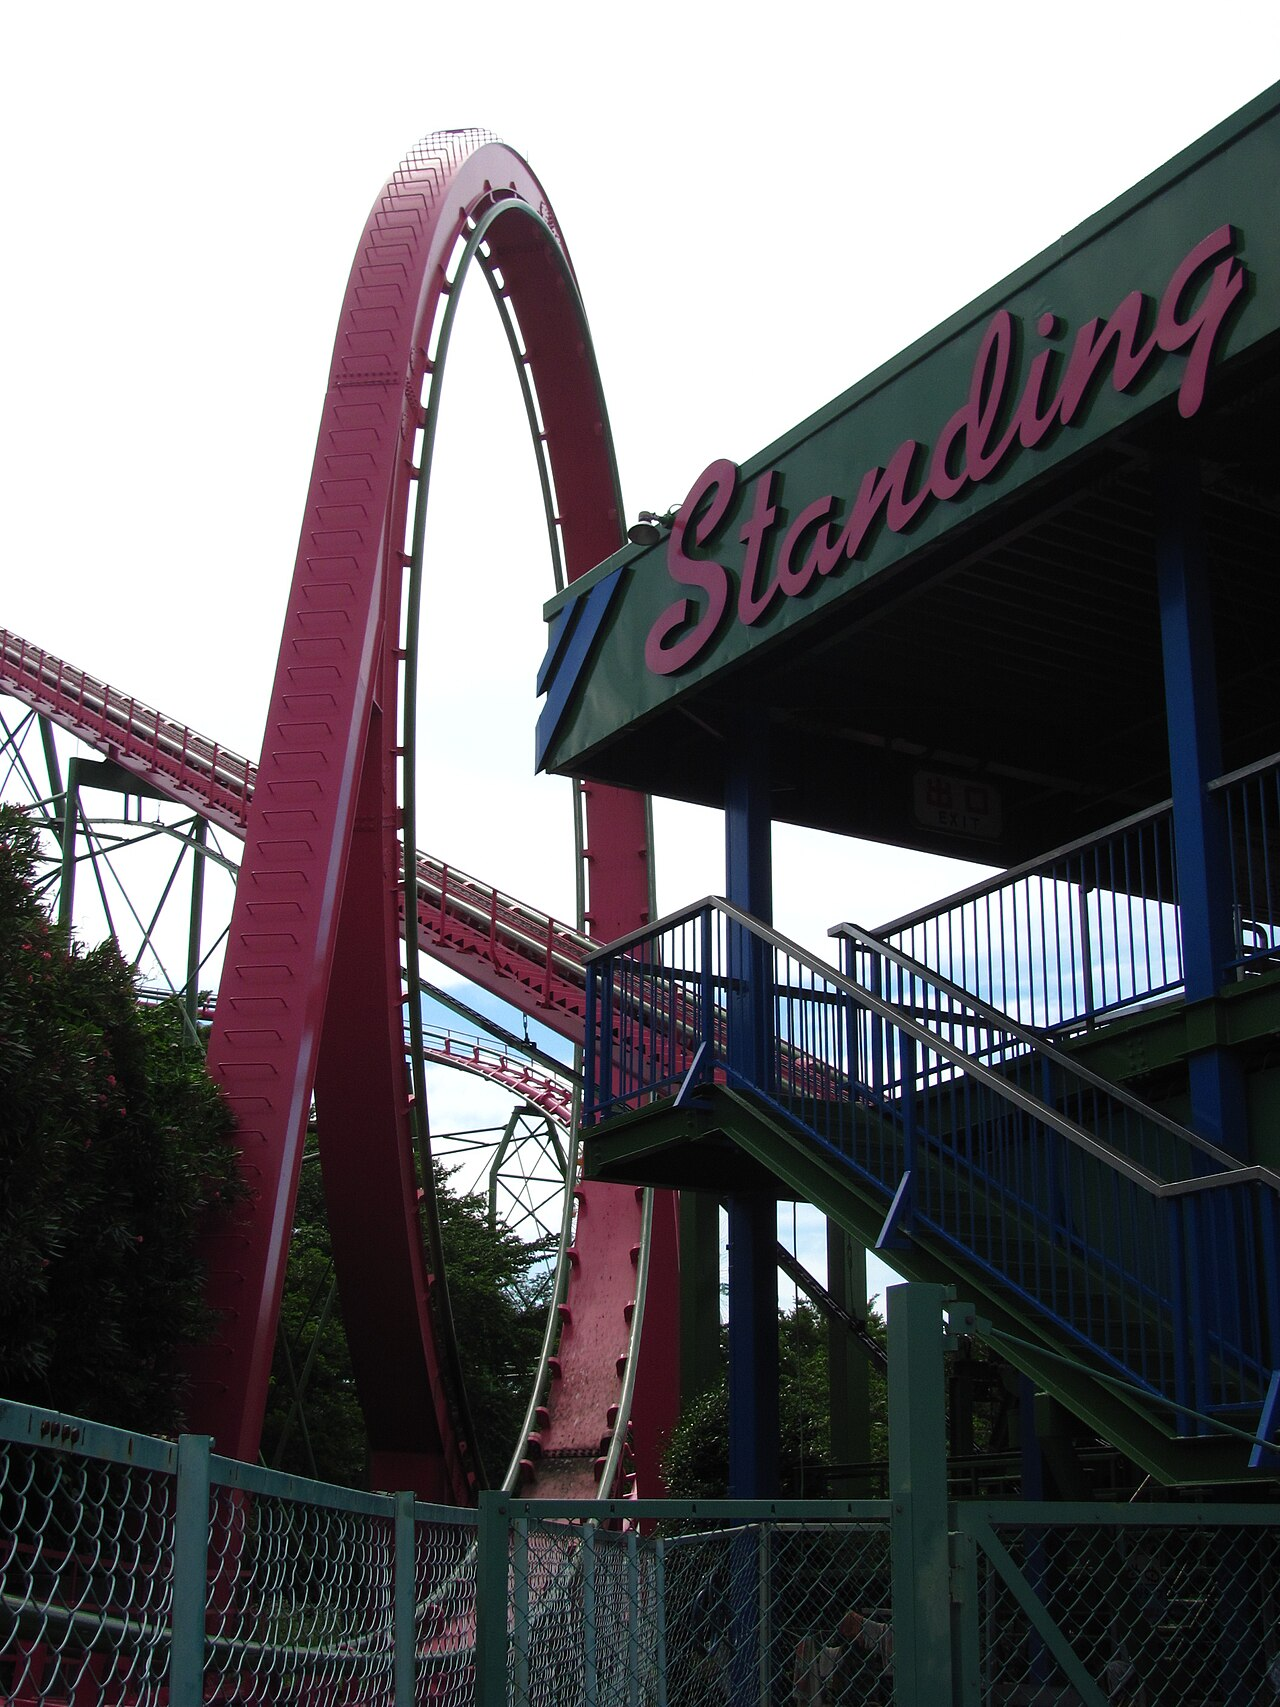
\includegraphics[width=0.38\linewidth]{images/book3/roller-coaster-loop.jpg}

{\small Un rizo vertical (Yomiuriland, Tokio): una lágrima antes que una circunferencia, para que la curvatura sea máxima arriba, donde la rapidez es mínima --- la geometría del problema de fin de semana. Fotografía: Jeremy Thompson, CC~BY~2.0.}
\end{omfigure}

\section{Problema: el rizo de una montaña rusa}

\begin{problem}[{Problema de fin de semana --- un vagón entra en un rizo
vertical a noventa kilómetros por hora: dónde frena, hacia dónde apunta su
aceleración, cuántos $g$ sienten los pasajeros y por qué los rizos
modernos no son circunferencias}]
\label{pb:b1:point-kinematics:1}
Un vagón, tratado como un punto $M$, recorre un rizo circular vertical de
radio $R = \qty{10}{m}$ y centro $C$. Su posición viene dada por el ángulo
$\theta$ entre $\vect{CM}$ y la vertical descendente ($\theta =
0$ abajo, $\pi$ arriba). Se desprecia el rozamiento, y la ley de rapidez
(deducida en \cref{ch:b1:work-and-energy}) es
\[
v^2 = v_0^2 - 2gR(1 - \cos\theta),
\]
con $v_0 = \qty{25}{m/s}$ la rapidez abajo; $g = \qty{9.81}{m/s^2}$.

\medskip
\noindent\textbf{Parte I --- Cinemática sobre la circunferencia.}
\begin{enumerate}
  \item En \omterm{def:b1:point-kinematics:cylindrical}{coordenadas polares} centradas en $C$ (con $\vect e_r$ de $C$
        hacia $M$), escríbanse $\vect v$ y $\vect a$ para el movimiento
        sobre la circunferencia.
  \item Identifíquense los vectores de Frenet $\vect T$ y $\vect N$ en
        función de $\vect e_r$ y $\vect e_\theta$, y el \omterm{def:b1:point-kinematics:frenet}{radio de curvatura}.
  \item Calcúlese la rapidez arriba y en los puntos laterales
        $\theta = \pi/2$ y $3\pi/2$.
  \item Derívese la ley de rapidez respecto del tiempo para mostrar que la
        \omterm{thm:b1:point-kinematics:frenet}{aceleración tangencial} vale $a_T = -g\sin\theta$. Interprétese su
        signo en la subida y en la bajada.
  \item Exprésese la \omterm{thm:b1:point-kinematics:frenet}{aceleración normal} $a_N(\theta)$ y calcúlese abajo,
        en los laterales y arriba.
  \item Dense la norma de $\vect a$ en los cuatro puntos y el ángulo que
        forma con la vertical en lo alto.
  \item ¿En qué puntos es $\vect a$ perpendicular a $\vect v$? ¿Y paralela?
\end{enumerate}

\medskip
\noindent\textbf{Parte II --- \omterm{cor:b1:point-kinematics:circular}{Velocidades angulares} y tiempos.}
\begin{enumerate}[resume]
  \item Exprésese $\dot\theta$ en función de $\theta$ y calcúlese abajo y
        arriba.
  \item Muéstrese que $\ddot\theta = -(g/R)\sin\theta$ (la ecuación de un
        péndulo) y coméntese.
  \item A modo de comparación, calcúlese el periodo de las pequeñas
        oscilaciones de un péndulo simple de longitud $R$
        (\cref{ex:b1:units-dimensions:pendulum} dio su forma; $k = 2\pi$).
  \item Estímese el tiempo que se tarda en recorrer el rizo, usando la
        media de las rapideces en los cuatro puntos de referencia.
  \item La rapidez mínima en lo alto para que el vagón no se despegue de
        la vía (capítulo siguiente) es $\sqrt{gR}$. ¿Se cumple? ¿Qué $v_0$
        mínima haría falta?
\end{enumerate}

\medskip
\noindent\textbf{Parte III --- Lo que sienten los pasajeros.}
El peso aparente por unidad de masa que siente un pasajero vale
$\vect a - \vect g$ (admitido aquí, deducido en
\cref{ch:b1:newton-dynamics}); su norma en unidades de $g$ es la ``carga en $g$''.
\begin{enumerate}[resume]
  \item Calcúlese la carga en $g$ abajo.
  \item Calcúlese arriba y dígase contra qué queda apretado el pasajero
        (el asiento o el arnés).
  \item Calcúlese en los puntos laterales.
  \item Los pasajeros toleran unos $4g$ durante poco tiempo. ¿Pasa la
        prueba este rizo? ¿Dónde está el problema?
  \item Muéstrese que, para un rizo circular tomado justo con la rapidez
        necesaria para superar lo alto (peso aparente nulo allí), la carga
        en $g$ abajo vale necesariamente $6g$, sea cual sea $R$.
\end{enumerate}

\medskip
\noindent\textbf{Parte IV --- El rizo en clotoide.}
Los rizos modernos tienen forma de lágrima: el \omterm{def:b1:point-kinematics:frenet}{radio de curvatura} es
grande abajo y pequeño arriba.
\begin{enumerate}[resume]
  \item Usando la forma de Frenet de $\vect a$, explíquese por qué variar
        $\rho$ a lo largo de la vía cambia $a_N$ sin cambiar la ley de
        rapidez (que solo depende de la altura).
  \item Elíjase $\rho_{\text{abajo}}$ para que la carga en $g$ abajo sea
        de $3g$ con $v_0 = \qty{25}{m/s}$.
  \item Arriba, la altura sigue siendo $2R = \qty{20}{m}$ sobre el punto
        más bajo. Elíjase $\rho_{\text{arriba}}$ para que la carga en $g$
        allí sea de $1.5g$.
  \item Una clotoide tiene la curvatura proporcional a la longitud de
        arco, $1/\rho = s/A^2$. A lo largo de una entrada así, con la
        rapidez casi constante, ¿cómo crece $a_N$ con el tiempo, y por qué
        resulta más suave para el cuello que una circunferencia (donde
        $a_N$ salta en la entrada)?
  \item Esbócese cualitativamente la forma del rizo resultante y
        resúmase en dos frases por qué sustituyó a la circunferencia.
\end{enumerate}

\medskip
\noindent\textbf{Parte V --- Visto desde el suelo.}
Una cámara a ras de suelo, a \qty{50}{m} del centro del rizo y en su
plano, sigue al vagón.
\begin{enumerate}[resume]
  \item Cuando el vagón está arriba y se mueve horizontalmente a
        \qty{15}{m/s}, ¿a qué \omterm{cor:b1:point-kinematics:circular}{velocidad angular} (rad/s) debe girar la
        cámara? (\omterm{def:b1:point-kinematics:cylindrical}{Coordenadas polares} desde la cámara.)
  \item ¿Por qué una cámara que gira a \omterm{def:b1:point-kinematics:velocity}{velocidad} constante sigue mal un
        \omterm{cor:b1:point-kinematics:circular}{movimiento circular} uniforme?
  \item Resúmase la lección del rizo para el capítulo: qué sistema de
        coordenadas respondió a cada pregunta.
\end{enumerate}
\end{problem}
